\documentclass[11pt,a4paper]{article}

% ==============================================================================
% PACKAGES & SYSTEM CONFIGURATION
% ==============================================================================
\usepackage[utf8]{inputenc}
\usepackage[T1]{fontenc}
\usepackage{lmodern}
\usepackage[margin=1in,headheight=14pt]{geometry}
\usepackage{microtype}
\usepackage{amsmath,amssymb}
\usepackage{booktabs}
\usepackage{tabularx}
\usepackage{longtable}
\usepackage{array}
\usepackage{float}
\usepackage{enumitem}
\usepackage{xcolor}
\usepackage{tikz}
\usetikzlibrary{shapes.geometric,arrows.meta,positioning,calc,fit,backgrounds}
\usepackage{tcolorbox}
\tcbuselibrary{skins,breakable}
\usepackage{fancyhdr}
\usepackage{titlesec}
\usepackage{cite}

% Hyperref setup
\usepackage[
    colorlinks=true,
    linkcolor=midnightblue,
    citecolor=teal,
    urlcolor=primary,
    bookmarks=true,
    bookmarksnumbered=true,
    pdfauthor={Abu Zafor, Anamul Haque},
    pdftitle={UniExpert - Software Requirements Specification (SRS)},
    pdfsubject={SE 331 Software Engineering Design Capstone Project},
    pdfkeywords={SRS, Requirements Engineering, IEEE 830, UniExpert, AI Matchmaking}
]{hyperref}

% ==============================================================================
% COLOR PALETTE (Academic & Clean)
% ==============================================================================
\definecolor{primary}{RGB}{20, 50, 95}       % Deep Academic Navy
\definecolor{secondary}{RGB}{40, 110, 180}   % Muted Steel Blue
\definecolor{accent}{RGB}{210, 105, 30}      % Subdued Terracotta
\definecolor{darkslate}{RGB}{35, 45, 55}     % Body Dark Gray
\definecolor{midnightblue}{RGB}{15, 35, 75}  % Header Blue
\definecolor{lightbg}{RGB}{247, 249, 252}    % Soft Gray Tint
\definecolor{bordercolor}{RGB}{215, 222, 232}% Card Border
\definecolor{tagmust}{RGB}{220, 53, 69}      % MoSCoW Must
\definecolor{tagshould}{RGB}{255, 140, 0}    % MoSCoW Should
\definecolor{tagcould}{RGB}{40, 167, 69}     % MoSCoW Could

% ==============================================================================
% CUSTOM BOXES & ENVIRONMENTS
% ==============================================================================
\newtcolorbox{reqbox}[2]{
    enhanced,
    colback=lightbg,
    colframe=secondary,
    coltitle=white,
    fonttitle=\bfseries\small,
    title={#1: #2},
    arc=2mm,
    boxrule=0.8pt,
    left=3mm,right=3mm,top=2mm,bottom=2mm,
    breakable
}

\newtcolorbox{calloutbox}[1]{
    enhanced,
    colback=lightbg,
    colframe=primary,
    coltitle=white,
    fonttitle=\bfseries\small,
    title={#1},
    arc=2mm,
    boxrule=1pt,
    left=3mm,right=3mm,top=2mm,bottom=2mm,
    breakable
}

% ==============================================================================
% SECTION FORMATTING
% ==============================================================================
\titleformat{\section}
  {\normalfont\Large\bfseries\color{primary}}{\thesection}{1em}{}[\titlerule]
\titleformat{\subsection}
  {\normalfont\large\bfseries\color{secondary}}{\thesubsection}{1em}{}
\titleformat{\subsubsection}
  {\normalfont\normalsize\bfseries\color{darkslate}}{\thesubsubsection}{1em}{}

% Header and Footer
\pagestyle{fancy}
\fancyhf{}
\fancyhead[L]{\small\color{gray}\textbf{UniExpert} $|$ Software Requirements Specification (SRS)}
\fancyhead[R]{\small\color{gray}SE 331 Capstone Project}
\fancyfoot[L]{\small\color{gray}Department of Software Engineering}
\fancyfoot[R]{\small\color{gray}\thepage}
\renewcommand{\headrulewidth}{0.4pt}
\renewcommand{\footrulewidth}{0.4pt}

% ==============================================================================
% DOCUMENT BEGINS
% ==============================================================================
\begin{document}

% ------------------------------------------------------------------------------
% MINIMAL COVER PAGE (Title Page)
% ------------------------------------------------------------------------------
\begin{titlepage}
    \centering
    \vspace*{1.2cm}
    
    {\large\scshape Department of Software Engineering}\\[0.2cm]
    {\normalsize Faculty of Science \& Information Technology}\\[2.2cm]
    
    {\Huge\bfseries\color{primary} UniExpert}\\[0.5cm]
    {\LARGE\bfseries\color{darkslate} AI-Powered Expert Discovery and Academic Collaboration Platform}\\[0.8cm]
    {\large\color{secondary} Software Requirements Specification (SRS)}\\[0.2cm]
    {\normalsize\textit{Standard Conforming to IEEE Std 830-1998 / ISO/IEC/IEEE 29148:2018}}\\[0.4cm]
    \rule{3.2in}{0.5pt}\\[0.6cm]
    
    {\normalsize\textbf{Course:} SE 331 --- Software Engineering Design Capstone Project}\\[0.25cm]
    {\normalsize\textbf{Semester:} Fall 2026 \quad $\cdot$ \quad \textbf{Duration:} October -- December 2026}\\[3.2cm]
    
    \begin{minipage}[t]{0.48\textwidth}
        \begin{flushleft}
            {\small\scshape Prepared By (Student Team)}\\[0.35cm]
            \textbf{Abu Zafor}\\
            {\small Student ID: 232-35-331}\\[0.25cm]
            \textbf{Anamul Haque}\\
            {\small Student ID: 232-35-285}
        \end{flushleft}
    \end{minipage}
    \hfill
    \begin{minipage}[t]{0.45\textwidth}
        \begin{flushright}
            {\small\scshape Supervised By}\\[0.35cm]
            \textbf{Mr. Md. Shohel Arman}\\[0.12cm]
            {\small Assistant Professor}\\
            {\small Department of Software Engineering}
        \end{flushright}
    \end{minipage}
    
    \vfill
    
    {\small\textbf{Date of Submission:} October 12, 2026}
    \vspace*{1.0cm}
\end{titlepage}

% ------------------------------------------------------------------------------
% DOCUMENT CONTROL & APPROVAL TABLE
% ------------------------------------------------------------------------------
\thispagestyle{plain}
\section*{Document Control and Revision History}
\addcontentsline{toc}{section}{Document Control and Revision History}

\begin{table}[H]
\centering
\small
\begin{tabularx}{\textwidth}{@{}l l l X l@{}}
\toprule
\textbf{Version} & \textbf{Date} & \textbf{Author(s)} & \textbf{Summary of Major Changes} & \textbf{Status} \\
\midrule
0.1 & Oct 02, 2026 & A. Zafor, A. Haque & Initial requirements elicitation and scope drafting. & Draft \\
0.5 & Oct 07, 2026 & A. Zafor, A. Haque & Complete IEEE 830 functional and non-functional requirements. & Reviewed \\
1.0 & Oct 12, 2026 & A. Zafor, A. Haque & Baseline SRS document submitted for Capstone committee review. & Approved \\
\bottomrule
\end{tabularx}
\end{table}

\vspace{0.6cm}
\begin{table}[H]
\centering
\small
\begin{tabularx}{\textwidth}{@{}l X l l@{}}
\toprule
\textbf{Role} & \textbf{Name \& Title} & \textbf{Affiliation} & \textbf{Signature / Date} \\
\midrule
Lead Author & Abu Zafor (Student ID: 232-35-331) & Dept. of Software Engineering & Verified / Oct 12, 2026 \\
Co-Author & Anamul Haque (Student ID: 232-35-285) & Dept. of Software Engineering & Verified / Oct 12, 2026 \\
Faculty Supervisor & Mr. Md. Shohel Arman (Assistant Professor) & Dept. of Software Engineering & Verified / Oct 12, 2026 \\
\bottomrule
\end{tabularx}
\end{table}

\vspace{0.8cm}
\begin{calloutbox}{Executive Specification Overview}
This Software Requirements Specification (SRS) establishes the formal baseline for the engineering, verification, and evaluation of \textbf{UniExpert}. UniExpert is an intelligent web-based discovery platform engineered to resolve the pervasive academic silo challenge in higher education. It parses natural language student research proposals, extracts skill entities via zero-shot transformer classifiers, indexes multi-modal expert profiles via dense embeddings in vector databases, executes multi-criteria hybrid ranking, and coordinates stateful collaboration lifecycles.
\end{calloutbox}

\newpage
% ------------------------------------------------------------------------------
% TABLE OF CONTENTS & LISTS
% ------------------------------------------------------------------------------
\tableofcontents
\vspace{0.5cm}
\listoffigures
\vspace{0.5cm}
\listoftables
\newpage

% ------------------------------------------------------------------------------
% SECTION 1: INTRODUCTION
% ------------------------------------------------------------------------------
\section{Introduction}

\subsection{Purpose of the Document}
The purpose of this Software Requirements Specification (SRS) document is to provide a complete, rigorous, and unambiguous description of the software requirements for \textbf{UniExpert} (AI-Powered Expert Discovery and Academic Collaboration Platform). This document specifies both functional and non-functional requirements, external interfaces, system constraints, domain models, and validation criteria. It serves as the formal contractual baseline between the student engineering team, the academic supervisor Mr. Md. Shohel Arman, and the capstone review committee for course \textbf{SE 331 (Software Engineering Design Capstone Project)} during the Fall 2026 semester.

\subsection{Document Conventions}
This SRS conforms to the IEEE Std 830-1998 and ISO/IEC/IEEE 29148:2018 guidelines. The following conventions are used throughout:
\begin{itemize}[noitemsep]
    \item \textbf{Requirement Identifiers:} Functional requirements are designated with the prefix \texttt{FR-[Module]-[Number]} (e.g., \texttt{FR-AUTH-01}).
    \item \textbf{Non-Functional Identifiers:} Non-functional requirements are designated with the prefix \texttt{NFR-[Category]-[Number]} (e.g., \texttt{NFR-PERF-01}).
    \item \textbf{Priority Tags:} Prioritization follows the MoSCoW framework:
    \begin{itemize}[noitemsep]
        \item \textbf{[M]} \textit{Must-Have:} Mandatory core functionality for the Minimum Viable Product (MVP).
        \item \textbf{[S]} \textit{Should-Have:} High-priority capabilities required for comprehensive evaluation.
        \item \textbf{[C]} \textit{Could-Have:} Desirable enhancements targeted if time and compute permit.
        \item \textbf{[W]} \textit{Won't-Have (this release):} Explicitly deferred out-of-scope capabilities.
    \end{itemize}
    \item \textbf{Normative Keywords:} The key words \textbf{SHALL}, \textbf{SHOULD}, and \textbf{MAY} are interpreted in accordance with RFC 2119.
\end{itemize}

\subsection{Intended Audience and Reading Suggestions}
This document is structured for the following stakeholders:
\begin{itemize}[noitemsep]
    \item \textbf{Capstone Evaluation Committee:} Focus on Section~\ref{sec:overall_desc} (Product Functions), Section~\ref{sec:functional_reqs} (System Features), and Section~\ref{sec:traceability} (Traceability).
    \item \textbf{Software Architects and Developers:} Focus on Section~\ref{sec:interfaces} (External Interfaces), Section~\ref{sec:functional_reqs} (Requirements Cards), and Section~\ref{sec:data_reqs} (Data Models).
    \item \textbf{Quality Assurance and Testers:} Focus on Section~\ref{sec:nfrs} (Non-Functional Benchmarks) and Section~\ref{sec:vv_plan} (Verification and Validation Plan).
\end{itemize}

\subsection{Project Scope}
The UniExpert platform addresses the systemic problem in university environments where students undertaking capstone projects, theses, and interdisciplinary research struggle to discover and initiate collaboration with qualified academic and industry mentors. UniExpert transforms expert discovery from a rigid keyword search into a problem-first, natural language workflow.

The core objectives of the system are:
\begin{enumerate}[label=\textbf{(\arabic*)},noitemsep]
    \item Ingest unstructured, natural language project statements submitted by students.
    \item Automatically extract domain classifications, technical skill prerequisites, and research scopes using zero-shot NLP models.
    \item Maintain a verified, multi-tier corpus of faculty, graduate researchers, and industry specialists.
    \item Compute multi-criteria compatibility scores combining semantic cosine similarity, skill taxonomy overlap, research interest alignment, credential authority, and schedule availability.
    \item Produce human-interpretable Explainable AI (XAI) justifications for every recommendation.
    \item Form multidisciplinary advisory teams using set-cover optimization to detect and resolve team skill gaps.
    \item Enforce a stateful collaboration lifecycle through an auditable Finite State Machine (FSM).
\end{enumerate}

\subsection{Definitions, Acronyms, and Abbreviations}
Table~\ref{tab:glossary} defines the domain-specific terms and acronyms utilized in this specification.

\begin{table}[H]
\centering
\small
\caption{Glossary of Technical Terms and Acronyms}
\label{tab:glossary}
\begin{tabularx}{\textwidth}{@{}l p{4.2cm} X@{}}
\toprule
\textbf{Term / Acronym} & \textbf{Full Expansion} & \textbf{Operational Definition in UniExpert} \\
\midrule
\textbf{SRS} & Software Requirements Specification & This formal specification document. \\
\textbf{EFS} & Expert Finding System & An information retrieval system that identifies people with expertise in a topic. \\
\textbf{HNSW} & Hierarchical Navigable Small World & Graph-based indexing algorithm used in Qdrant for approximate nearest neighbor vector search. \\
\textbf{XAI} & Explainable Artificial Intelligence & Subsystem that articulates human-readable rationales for expert recommendations. \\
\textbf{FSM} & Finite State Machine & Formal state transition model governing collaboration proposals. \\
\textbf{RBAC} & Role-Based Access Control & Authorization framework governing students, experts, and administrators. \\
\textbf{BM25} & Best Matching 25 & Classical probabilistic keyword retrieval ranking function used as baseline. \\
\textbf{NDCG} & Normalized Discounted Cumulative Gain & Standard ranking metric assessing recommendation quality graded by relevance. \\
\textbf{ORCID} & Open Researcher and Contributor ID & Persistent digital identifier disambiguating academic authors. \\
\textbf{JWT} & JSON Web Token & Compact, URL-safe means of representing claims between two parties. \\
\bottomrule
\end{tabularx}
\end{table}

\subsection{References}
\begin{enumerate}[label={[\arabic*]},noitemsep]
    \item IEEE Computer Society, \emph{IEEE Std 830-1998: IEEE Recommended Practice for Software Requirements Specifications}, IEEE, 1998.
    \item ISO/IEC/IEEE, \emph{ISO/IEC/IEEE 29148:2018 Systems and Software Engineering --- Life Cycle Processes --- Requirements Engineering}, 2018.
    \item K.~Balog, \emph{Expertise Retrieval: A Survey}, Foundations and Trends in Information Retrieval, vol.~6, no.~2--3, pp.~127--256, 2012.
    \item N.~Reimers and I.~Gurevych, \emph{Sentence-BERT: Sentence Embeddings using Siamese BERT-Networks}, in Proc. EMNLP 2019.
\end{enumerate}

\clearpage
% ------------------------------------------------------------------------------
% SECTION 2: OVERALL DESCRIPTION
% ------------------------------------------------------------------------------
\section{Overall Description}
\label{sec:overall_desc}

\subsection{Product Perspective}
UniExpert is a self-contained, cloud-deployable web application with dedicated external interfaces to university identity providers, public academic bibliometric repositories (ORCID, Google Scholar), and enterprise SMTP services. The system operates in a multi-tier microservice-inspired architecture, decoupling the compute-intensive AI inference pipeline from user-facing CRUD workloads.

\begin{figure}[H]
\centering
\resizebox{0.95\linewidth}{!}{%
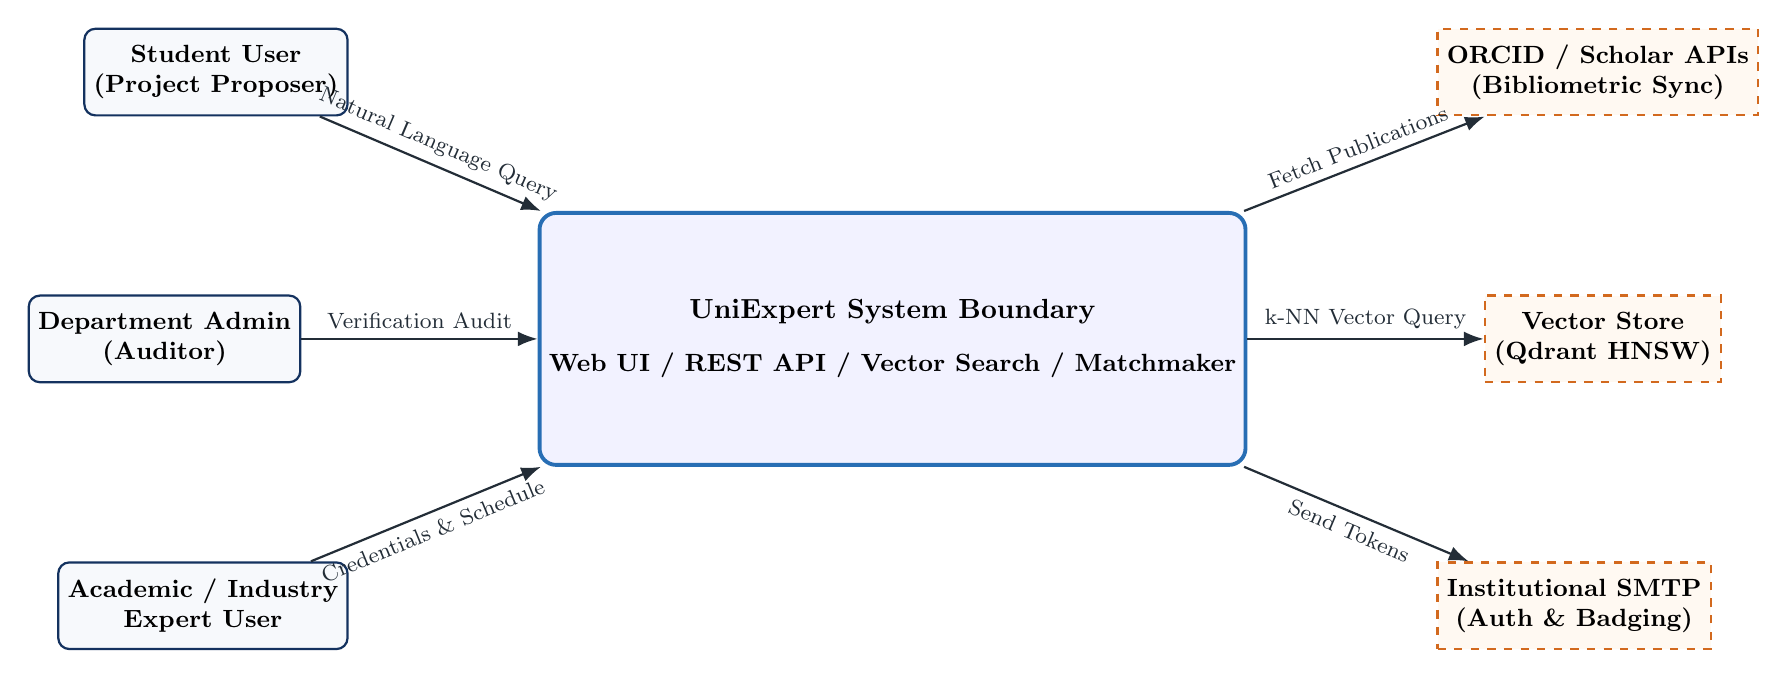
\begin{tikzpicture}[
    actor/.style={rectangle, draw=primary, fill=lightbg, rounded corners=4pt, thick, align=center, font=\small\bfseries, minimum height=1.1cm, minimum width=2.8cm},
    system/.style={rectangle, draw=secondary, fill=blue!5, rounded corners=6pt, line width=1.4pt, align=center, font=\normalsize\bfseries, minimum height=3.2cm, minimum width=6.8cm},
    ext/.style={rectangle, draw=accent, fill=orange!5, dashed, thick, align=center, font=\small\bfseries, minimum height=1.1cm, minimum width=2.8cm},
    conn/.style={-{Latex[length=2.5mm]}, thick, color=darkslate}
]

    % Core UniExpert System
    \node[system] (core) {\textbf{UniExpert System Boundary}\\[0.25cm]\small Web UI / REST API / Vector Search / Matchmaker};

    % Actors (Left side with clean separation)
    \node[actor, above left=1.2cm and 2.4cm of core] (student) {Student User\\(Project Proposer)};
    \node[actor, below left=1.2cm and 2.4cm of core] (expert) {Academic / Industry\\Expert User};
    \node[actor, left=3.0cm of core] (admin) {Department Admin\\(Auditor)};

    % External Systems (Right side with clean separation)
    \node[ext, above right=1.2cm and 2.4cm of core] (orcid) {ORCID / Scholar APIs\\(Bibliometric Sync)};
    \node[ext, below right=1.2cm and 2.4cm of core] (smtp) {Institutional SMTP\\(Auth \& Badging)};
    \node[ext, right=3.0cm of core] (qdrant) {Vector Store\\(Qdrant HNSW)};

    % Data Flows
    \draw[conn] (student) -- node[above,sloped,font=\footnotesize] {Natural Language Query} (core.160);
    \draw[conn] (expert) -- node[below,sloped,font=\footnotesize] {Credentials \& Schedule} (core.200);
    \draw[conn] (admin) -- node[above,font=\footnotesize] {Verification Audit} (core.west);
    
    \draw[conn] (core.20) -- node[above,sloped,font=\footnotesize] {Fetch Publications} (orcid);
    \draw[conn] (core.340) -- node[below,sloped,font=\footnotesize] {Send Tokens} (smtp);
    \draw[conn] (core.east) -- node[above,font=\footnotesize] {k-NN Vector Query} (qdrant);

\end{tikzpicture}%
}
\caption{UniExpert System Context Diagram}
\label{fig:context_diagram}
\end{figure}

\subsection{Product Functions Overview}
Figure~\ref{fig:functional_tree} synthesizes the top-level functional hierarchy of UniExpert across its four core subsystems.

\begin{figure}[H]
\centering
\resizebox{0.98\linewidth}{!}{%
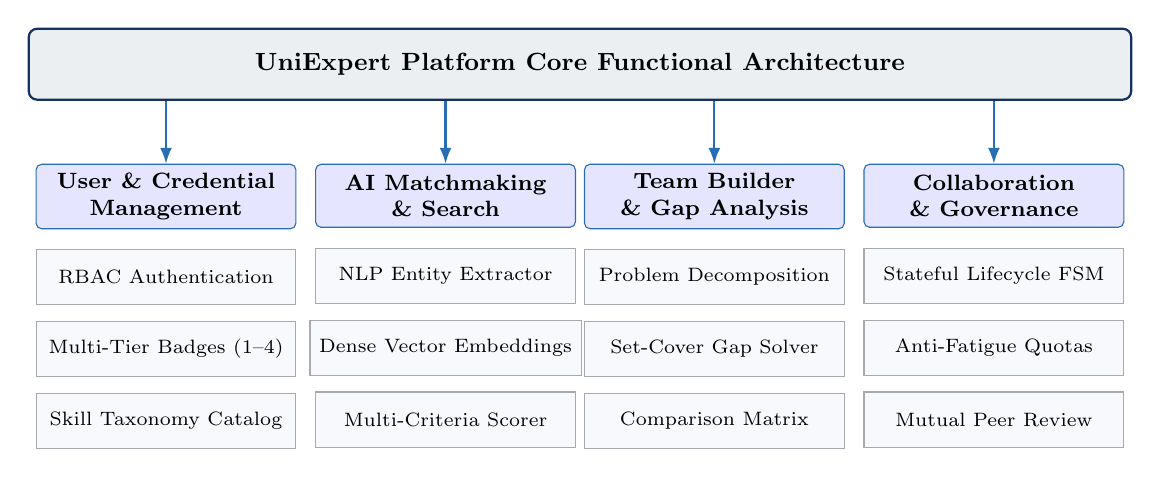
\begin{tikzpicture}[
    box/.style={rectangle, draw=primary, fill=primary!8, rounded corners=3pt, thick, align=center, font=\bfseries\small, minimum width=14cm, minimum height=0.9cm},
    colheader/.style={rectangle, draw=secondary, fill=blue!10, rounded corners=2pt, font=\bfseries\footnotesize, align=center, minimum width=3.3cm, minimum height=0.8cm},
    subbox/.style={rectangle, draw=darkslate!40, fill=lightbg, font=\scriptsize, align=center, minimum width=3.3cm, minimum height=0.7cm},
    arr/.style={-{Latex[length=2mm]}, thick, color=secondary}
]
    % Root
    \node[box] (root) {\textbf{UniExpert Platform Core Functional Architecture}};

    % Column 1: Auth & Identity
    \node[colheader, below left=0.8cm and 3.6cm of root.south] (col1) {User \& Credential\\Management};
    \node[subbox, below=0.25cm of col1] (s11) {RBAC Authentication};
    \node[subbox, below=0.2cm of s11] (s12) {Multi-Tier Badges (1--4)};
    \node[subbox, below=0.2cm of s12] (s13) {Skill Taxonomy Catalog};

    % Column 2: AI Matchmaking
    \node[colheader, below left=0.8cm and 0.05cm of root.south] (col2) {AI Matchmaking\\\& Search};
    \node[subbox, below=0.25cm of col2] (s21) {NLP Entity Extractor};
    \node[subbox, below=0.2cm of s21] (s22) {Dense Vector Embeddings};
    \node[subbox, below=0.2cm of s22] (s23) {Multi-Criteria Scorer};

    % Column 3: Team Builder
    \node[colheader, below right=0.8cm and 0.05cm of root.south] (col3) {Team Builder\\\& Gap Analysis};
    \node[subbox, below=0.25cm of col3] (s31) {Problem Decomposition};
    \node[subbox, below=0.2cm of s31] (s32) {Set-Cover Gap Solver};
    \node[subbox, below=0.2cm of s32] (s33) {Comparison Matrix};

    % Column 4: Collaboration
    \node[colheader, below right=0.8cm and 3.6cm of root.south] (col4) {Collaboration\\\& Governance};
    \node[subbox, below=0.25cm of col4] (s41) {Stateful Lifecycle FSM};
    \node[subbox, below=0.2cm of s41] (s42) {Anti-Fatigue Quotas};
    \node[subbox, below=0.2cm of s42] (s43) {Mutual Peer Review};

    % Connectors
    \draw[arr] (root.south -| col1.north) -- (col1.north);
    \draw[arr] (root.south -| col2.north) -- (col2.north);
    \draw[arr] (root.south -| col3.north) -- (col3.north);
    \draw[arr] (root.south -| col4.north) -- (col4.north);

\end{tikzpicture}%
}
\caption{UniExpert Functional Subsystem Architecture}
\label{fig:functional_tree}
\end{figure}

\subsection{User Classes and Characteristics}
UniExpert serves four distinct categories of users with varying privileges and operational objectives, summarized in Table~\ref{tab:user_classes}.

\begin{table}[H]
\centering
\small
\caption{User Classes and Operational Profiles}
\label{tab:user_classes}
\begin{tabularx}{\textwidth}{@{}p{3.2cm} p{2.8cm} X l@{}}
\toprule
\textbf{User Class} & \textbf{Technical Profile} & \textbf{Key Responsibilities \& Permissions} & \textbf{Frequency} \\
\midrule
\textbf{Student Researcher} & Moderate web familiarity; novice in taxonomy & Submits project proposals; reviews AI recommendations; creates multidisciplinary teams; sends collaboration requests. & Daily during semester \\
\addlinespace
\textbf{Academic Expert} (Professor / Researcher) & High academic domain expertise & Publishes research skills; toggles availability blackouts; reviews project requests; collaborates in workspaces. & Weekly \\
\addlinespace
\textbf{Industry Mentor} & High professional software / engineering skill & Offers industry perspective; sets consultation capacity; evaluates applied capstone feasibility. & Bi-weekly \\
\addlinespace
\textbf{Department Admin} & High technical and administrative authorization & Verifies institutional documentation; resolves user disputes; inspects system telemetry and IR performance. & Periodic \\
\bottomrule
\end{tabularx}
\end{table}

\subsection{Operating Environment}
The software shall operate reliably within the following environments:
\begin{itemize}[noitemsep]
    \item \textbf{Client-Side:} Modern evergreen web browsers (Chromium $\ge 118$, Mozilla Firefox $\ge 120$, Apple Safari $\ge 17$, Microsoft Edge $\ge 118$) across desktop, tablet, and mobile displays.
    \item \textbf{Backend Server:} Linux OS (Ubuntu 22.04 LTS or Debian 12) running Python 3.11+ ASGI asynchronous web services (FastAPI / Uvicorn).
    \item \textbf{Data Stores:} PostgreSQL 16 relational database with ACID guarantees; Qdrant 1.8+ dedicated vector database with HNSW cosine distance indexing; Redis 7.2 in-memory cache and rate-limit broker.
    \item \textbf{Virtualization \& Deployment:} Docker Engine 24.0+ and Docker Compose v2 for containerized local development and cloud production deployment.
\end{itemize}

\subsection{Design and Implementation Constraints}
\begin{enumerate}[label=\textbf{(\arabic*)},noitemsep]
    \item \textbf{Compute Constraints:} The AI inference engine must execute zero-shot skill extraction and embedding generation using CPU-optimized architectures (ONNX Runtime / FastEmbed) without requiring dedicated multi-GPU cloud instances.
    \item \textbf{Security \& Compliance:} Student email addresses, draft project concepts, and direct messages must be protected using TLS 1.3 in transit and AES-256 at rest, respecting FERPA guidelines.
    \item \textbf{Academic Integrity:} The system shall not write or synthesize academic project code or thesis literature; its sole AI function is discovery, entity extraction, ranking, and matchmaking.
    \item \textbf{Zero License Costs:} The platform must strictly utilize permissive open-source libraries (MIT, Apache 2.0, BSD) ensuring no proprietary licensing liabilities.
\end{enumerate}

\subsection{Assumptions and Dependencies}
\begin{itemize}[noitemsep]
    \item The university possesses an active SMTP relay or provides access to institutional email domains (\texttt{.edu}) for automated credential validation.
    \item Public research metadata can be harvested via open ORCID and Google Scholar endpoints within allowable rate limits.
    \item Participating experts voluntarily register and configure their availability status.
\end{itemize}

\clearpage
% ------------------------------------------------------------------------------
% SECTION 3: EXTERNAL INTERFACE REQUIREMENTS
% ------------------------------------------------------------------------------
\section{External Interface Requirements}
\label{sec:interfaces}

\subsection{User Interfaces (UI)}
The UniExpert graphical interface shall be designed according to modern usability principles (WCAG 2.1 AA compliance):
\begin{itemize}[noitemsep]
    \item \textbf{Design System:} Cohesive design system built with clean typography, responsive CSS Grid / Flexbox layouts, and high-contrast color tokens.
    \item \textbf{Responsive Breakpoints:} Desktop ($\ge 1200\text{px}$), Tablet ($768\text{px} - 1199\text{px}$), and Mobile ($< 768\text{px}$).
    \item \textbf{Interactive Views:}
    \begin{enumerate}[label=\textbf{(\alph*)},noitemsep]
        \item \textit{Project Ingestion Console:} Freeform rich-text input with live entity highlighting showing extracted skills and suggested taxonomy tags.
        \item \textit{Recommendation Explorer:} Side-by-side candidate cards displaying overall compatibility score, sub-scores, verified badges, and XAI justification tooltips.
        \item \textit{Team Assembly Workbench:} Visual drag-and-drop panel computing collective skill coverage in real-time.
        \item \textit{Collaboration FSM Dashboard:} Kanban-style visual pipeline representing sent, pending, accepted, and completed requests.
    \end{enumerate}
\end{itemize}

\subsection{Hardware Interfaces}
No dedicated proprietary hardware interfaces are required. The system communicates over standard TCP/IP networking hardware. Minimal recommended host hardware comprises:
\begin{itemize}[noitemsep]
    \item CPU: 4 vCPUs (x86-64 or ARM64 architecture).
    \item RAM: 8 GB memory minimum (16 GB recommended for high concurrent embedding loads).
    \item Storage: 40 GB NVMe SSD persistent storage for database volumes.
\end{itemize}

\subsection{Software Interfaces}
Table~\ref{tab:software_interfaces} enumerates all external and intra-system software interfaces.

\begin{table}[H]
\centering
\small
\caption{Software Interfaces and Protocols}
\label{tab:software_interfaces}
\begin{tabularx}{\textwidth}{@{}l l p{3.2cm} X@{}}
\toprule
\textbf{Component} & \textbf{Interface Type} & \textbf{Protocol / Format} & \textbf{Purpose and Payload} \\
\midrule
\textbf{PostgreSQL 16} & Relational DB & TCP / asyncpg / SQL & Stores user accounts, profiles, project records, reviews, and audit logs. \\
\addlinespace
\textbf{Qdrant Engine} & Vector Database & gRPC / REST / JSON & Stores 384-dimensional dense embeddings; executes cosine HNSW $k$-NN searches. \\
\addlinespace
\textbf{Redis 7} & In-Memory Store & TCP / RESP protocol & Manages active user sessions, token blocklists, and API rate-limiting buckets. \\
\addlinespace
\textbf{FastEmbed / ONNX} & Embedded ML & Python API & Generates \texttt{all-MiniLM-L6-v2} embeddings locally with sub-millisecond CPU latency. \\
\addlinespace
\textbf{ORCID API} & Public Web API & HTTPS / REST / JSON & Fetches public author publication histories, DOI lists, and institutional affiliations. \\
\addlinespace
\textbf{Mail Server} & Transactional Mail & SMTP / TLS (Port 587) & Dispatches account activation tokens, verification links, and invitation notifications. \\
\bottomrule
\end{tabularx}
\end{table}

\subsection{Communications Interfaces}
\begin{itemize}[noitemsep]
    \item \textbf{Client-Server Communication:} All web traffic shall be encrypted using TLS 1.3 over HTTPS. Unencrypted HTTP requests shall be rejected with HTTP 301 redirects.
    \item \textbf{API Communication:} RESTful endpoints follow JSON API conventions; API error responses adhere to RFC 7807 (Problem Details for HTTP APIs).
    \item \textbf{Real-Time Workspace Messaging:} Secured WebSockets (\texttt{wss://}) provide bi-directional event notifications for collaboration state transitions and instant chat updates.
\end{itemize}

\clearpage
% ------------------------------------------------------------------------------
% SECTION 4: SYSTEM FEATURES AND FUNCTIONAL REQUIREMENTS
% ------------------------------------------------------------------------------
\section{System Features and Functional Requirements}
\label{sec:functional_reqs}

This section details the 20 functional requirements grouped into 7 modular subsystems.

% ------------------------------------------------------------------------------
% MODULE 1: AUTH & RBAC
% ------------------------------------------------------------------------------
\subsection{Module 1: Authentication and Identity Management}

\begin{reqbox}{FR-AUTH-01}{User Registration and Institutional Verification}
\begin{tabularx}{\textwidth}{@{}lX@{}}
\textbf{Priority:} & \textbf{[M]} Must-Have \\
\textbf{Description:} & The system SHALL allow students, academic experts, and industry mentors to register unique accounts. Academic experts registering with an institutional email (\texttt{.edu} or departmental domain) SHALL automatically trigger an automated cryptographic activation token. \\
\textbf{Input:} & Full Name, Email, Password (min 10 chars, mixed case, numeric, special), User Role. \\
\textbf{Output:} & Account creation confirmation, verification email with expiring HMAC token (24-hour TTL). \\
\textbf{Precondition:} & Email address is not previously registered in the system. \\
\textbf{Postcondition:} & Unverified user record created in PostgreSQL with status \texttt{PENDING\_VERIFICATION}. \\
\end{tabularx}
\end{reqbox}

\begin{reqbox}{FR-AUTH-02}{Role-Based Access Control (RBAC) and Session Management}
\begin{tabularx}{\textwidth}{@{}lX@{}}
\textbf{Priority:} & \textbf{[M]} Must-Have \\
\textbf{Description:} & The system SHALL enforce strict RBAC across four distinct scopes: \texttt{STUDENT}, \texttt{EXPERT}, \texttt{ADMIN}, and \texttt{AUDITOR}. Sessions SHALL be maintained using short-lived JWT access tokens (15-minute TTL) and secure HTTP-only refresh tokens (7-day TTL). \\
\textbf{Input:} & User login credentials (Email, Password). \\
\textbf{Output:} & Access JWT with encoded scopes; refresh token stored in encrypted cookie. \\
\textbf{Precondition:} & User email has been verified. \\
\textbf{Postcondition:} & Authentication token issued; session logged with IP and User-Agent telemetry. \\
\end{tabularx}
\end{reqbox}

% ------------------------------------------------------------------------------
% MODULE 2: PROFILE & TAXONOMY
% ------------------------------------------------------------------------------
\subsection{Module 2: Profile Engineering and Taxonomy Management}

\begin{reqbox}{FR-PROF-03}{Student Academic Profile Management}
\begin{tabularx}{\textwidth}{@{}lX@{}}
\textbf{Priority:} & \textbf{[M]} Must-Have \\
\textbf{Description:} & The system SHALL provide students with a comprehensive profile dashboard capturing university name, student ID, department, current degree program, research interests, and previous project repositories. \\
\textbf{Input:} & Academic metadata, biography, CV attachment (PDF max 5MB), GitHub / LinkedIn URLs. \\
\textbf{Output:} & Rendered student profile card; searchable profile entity in database. \\
\textbf{Precondition:} & Authenticated with \texttt{STUDENT} role. \\
\textbf{Postcondition:} & Profile saved and associated with project listings. \\
\end{tabularx}
\end{reqbox}

\begin{reqbox}{FR-PROF-04}{Multi-Tier Expert Credential Verification Workflow}
\begin{tabularx}{\textwidth}{@{}lX@{}}
\textbf{Priority:} & \textbf{[M]} Must-Have \\
\textbf{Description:} & The system SHALL support a four-tier progressive verification badge framework:
\begin{enumerate}[noitemsep]
    \item \textbf{Tier 1 (Email):} Verified institutional \texttt{.edu} email.
    \item \textbf{Tier 2 (Bibliometric):} Verified ORCID ID with $\ge 2$ indexed publications.
    \item \textbf{Tier 3 (Institutional):} Departmental appointment letter reviewed by Admin.
    \item \textbf{Tier 4 (Industry):} Corporate domain email with verified professional credentials.
\end{enumerate} \\
\textbf{Input:} & Verification artifacts (ID card scan, appointment letter, ORCID token). \\
\textbf{Output:} & Public profile badges: \texttt{[Verified Faculty]}, \texttt{[Verified Researcher]}, \texttt{[Industry Mentor]}. \\
\textbf{Precondition:} & Authenticated with \texttt{EXPERT} role. \\
\textbf{Postcondition:} & Credential authority weight $\mathcal{V}(e)$ updated in ranking algorithm. \\
\end{tabularx}
\end{reqbox}

\begin{reqbox}{FR-PROF-05}{Hierarchical Academic Skill and Domain Taxonomy}
\begin{tabularx}{\textwidth}{@{}lX@{}}
\textbf{Priority:} & \textbf{[M]} Must-Have \\
\textbf{Description:} & The system SHALL maintain a structured, multi-level academic taxonomy spanning Computer Science, Software Engineering, Electrical Engineering, Biotechnology, Agriculture, Business, and Data Science. It SHALL support autocomplete and alias mapping (e.g., mapping ``CV'' to ``Computer Vision''). \\
\textbf{Input:} & Search keywords or taxonomy navigation queries. \\
\textbf{Output:} & Standardized taxonomy entity nodes with parent, child, and related skill links. \\
\textbf{Precondition:} & System taxonomy seeded in database. \\
\textbf{Postcondition:} & Query skill mapped to canonical taxonomy ID. \\
\end{tabularx}
\end{reqbox}

% ------------------------------------------------------------------------------
% MODULE 3: NLP EXTRACTION
% ------------------------------------------------------------------------------
\subsection{Module 3: Natural Language Problem Ingestion and NLP Extraction}

\begin{reqbox}{FR-NLP-06}{Unstructured Project Statement Ingestion}
\begin{tabularx}{\textwidth}{@{}lX@{}}
\textbf{Priority:} & \textbf{[M]} Must-Have \\
\textbf{Description:} & The system SHALL accept free-text project problem descriptions from students (minimum 50 words, maximum 2,000 words). The submission form SHALL accept project title, target domain, expected methodology, and project timeline. \\
\textbf{Input:} & Free-text research statement, target domain category, project type (Capstone, Thesis, Research). \\
\textbf{Output:} & Structured project record assigned a unique UUID. \\
\textbf{Precondition:} & Authenticated student user. \\
\textbf{Postcondition:} & Asynchronous NLP parsing event dispatched to background task worker. \\
\end{tabularx}
\end{reqbox}

\begin{reqbox}{FR-NLP-07}{Automated Skill and Domain Entity Extraction}
\begin{tabularx}{\textwidth}{@{}lX@{}}
\textbf{Priority:} & \textbf{[M]} Must-Have \\
\textbf{Description:} & The system SHALL parse project descriptions using zero-shot classification and dictionary-guided named entity recognition (NER). It SHALL extract: (1) Primary Domain; (2) Secondary Domains; (3) Core Technical Prerequisites; and (4) Methodological Paradigms. \\
\textbf{Input:} & Raw unstructured project text string. \\
\textbf{Output:} & JSON array of identified skills with confidence scores $\in [0, 1]$. \\
\textbf{Precondition:} & NLP model pipeline initialized and warm in memory. \\
\textbf{Postcondition:} & Extracted entities linked to project record in relational store. \\
\end{tabularx}
\end{reqbox}

\begin{reqbox}{FR-NLP-08}{Interactive Student Requirement Refinement}
\begin{tabularx}{\textwidth}{@{}lX@{}}
\textbf{Priority:} & \textbf{[S]} Should-Have \\
\textbf{Description:} & The system SHALL present extracted skills and domain tags to the student in an interactive confirmation interface. The student SHALL have the ability to remove spurious tags, adjust importance weights (Must-Have vs. Nice-to-Have), and manually append additional skills. \\
\textbf{Input:} & Student adjustments (tag deletions, additions, weight modifications). \\
\textbf{Output:} & Finalized requirement vector $\mathcal{K}_u$ with associated weights $w_k$. \\
\textbf{Precondition:} & Automated NLP extraction completed. \\
\textbf{Postcondition:} & Refined requirement vector committed as input to matchmaker. \\
\end{tabularx}
\end{reqbox}

% ------------------------------------------------------------------------------
% MODULE 4: MATCHING & XAI
% ------------------------------------------------------------------------------
\subsection{Module 4: Semantic Matching and Hybrid Recommendation Engine}

\begin{reqbox}{FR-REC-09}{Dense Semantic Embedding Generation and Vector Indexing}
\begin{tabularx}{\textwidth}{@{}lX@{}}
\textbf{Priority:} & \textbf{[M]} Must-Have \\
\textbf{Description:} & The system SHALL transform finalized project problem statements and expert research biographies into 384-dimensional dense semantic vectors using the \texttt{all-MiniLM-L6-v2} embedding model. Vectors SHALL be indexed in Qdrant with HNSW graphs ($M=16, \text{ef\_construct}=100$). \\
\textbf{Input:} & Canonical text representations of projects and expert profiles. \\
\textbf{Output:} & 384-dimensional unit-normalized embedding vector $\vec{v} \in \mathbb{R}^{384}$. \\
\textbf{Precondition:} & Text preprocessing and stop-word normalization executed. \\
\textbf{Postcondition:} & Vector stored in Qdrant collection with payload containing profile ID. \\
\end{tabularx}
\end{reqbox}

\begin{reqbox}{FR-REC-10}{Multi-Criteria Hybrid Scoring Engine}
\begin{tabularx}{\textwidth}{@{}lX@{}}
\textbf{Priority:} & \textbf{[M]} Must-Have \\
\textbf{Description:} & The system SHALL compute an overall composite compatibility score $\mathcal{S}(u, e) \in [0, 1]$ between student project $u$ and expert candidate $e$ using the formal multi-criteria formulation:
\begin{equation}
    \label{eq:srs_hybrid}
    \mathcal{S}(u, e) = w_1 \cdot \mathcal{D}(u, e) + w_2 \cdot \mathcal{K}(u, e) + w_3 \cdot \mathcal{R}(u, e) + w_4 \cdot \mathcal{V}(e) + w_5 \cdot \mathcal{A}(u, e)
\end{equation}
subject to $\sum_{i=1}^5 w_i = 1.0$ (baseline configuration: $w_1=0.30, w_2=0.25, w_3=0.20, w_4=0.15, w_5=0.10$). \\
\textbf{Input:} & Student project vector, extracted skill list, candidate expert profiles. \\
\textbf{Output:} & Ranked list of candidate experts ordered by descending $\mathcal{S}(u, e)$. \\
\textbf{Precondition:} & Candidate expert matches availability and domain criteria. \\
\textbf{Postcondition:} & Top-$K$ recommendations ($K=10$) rendered to student. \\
\end{tabularx}
\end{reqbox}

\begin{reqbox}{FR-REC-11}{Explainable AI (XAI) Justification Generation}
\begin{tabularx}{\textwidth}{@{}lX@{}}
\textbf{Priority:} & \textbf{[M]} Must-Have \\
\textbf{Description:} & For every recommended expert, the system SHALL synthesize a natural-language explanatory rationale detailing:
\begin{itemize}[noitemsep]
    \item Direct overlapping skill sets (e.g., ``Matches 4 out of 5 required skills: PyTorch, Computer Vision'').
    \item Relevant recent publications or project history aligned with the student's problem.
    \item Current availability status and preferred collaboration modes.
\end{itemize} \\
\textbf{Input:} & Sub-score breakdown from Equation~\ref{eq:srs_hybrid} and overlapping entity sets. \\
\textbf{Output:} & Human-readable justification card displayed beneath candidate card. \\
\textbf{Precondition:} & Hybrid score calculated. \\
\textbf{Postcondition:} & Explanatory metadata cached for frontend rendering. \\
\end{tabularx}
\end{reqbox}

\begin{reqbox}{FR-REC-12}{Dynamic Faceted Filtering and Re-ranking}
\begin{tabularx}{\textwidth}{@{}lX@{}}
\textbf{Priority:} & \textbf{[M]} Must-Have \\
\textbf{Description:} & The system SHALL allow students to dynamically filter and re-rank candidate recommendations by: minimum verification tier, academic vs. industry affiliation, current mentoring availability, and specific domain tags without re-invoking the full embedding pipeline. \\
\textbf{Input:} & Filter predicate parameters (e.g., \texttt{min\_tier=2}, \texttt{is\_available=true}). \\
\textbf{Output:} & Instantaneously updated recommendation list adhering to filter constraints. \\
\textbf{Precondition:} & Initial candidate recommendation set retrieved. \\
\textbf{Postcondition:} & Filtered results displayed in $< 100\text{ms}$. \\
\end{tabularx}
\end{reqbox}

% ------------------------------------------------------------------------------
% MODULE 5: TEAM BUILDER & GAP ANALYSIS
% ------------------------------------------------------------------------------
\subsection{Module 5: Multidisciplinary Team Formation and Gap Analysis}

\begin{reqbox}{FR-TEAM-13}{Multidisciplinary Project Decomposition}
\begin{tabularx}{\textwidth}{@{}lX@{}}
\textbf{Priority:} & \textbf{[S]} Should-Have \\
\textbf{Description:} & When a project is classified as interdisciplinary (e.g., AI in Poultry Farming), the system SHALL automatically decompose the requirements into discrete sub-domains (e.g., Sub-domain A: Computer Vision; Sub-domain B: Veterinary Pathology). \\
\textbf{Input:} & Interdisciplinary project description. \\
\textbf{Output:} & Decomposed sub-domain requirement tuples $(D_1, \mathcal{K}_1), (D_2, \mathcal{K}_2)$. \\
\textbf{Precondition:} & Project requirements contain multiple disparate high-level ontology roots. \\
\textbf{Postcondition:} & Dedicated recommendation tracks generated for each sub-domain. \\
\end{tabularx}
\end{reqbox}

\begin{reqbox}{FR-TEAM-14}{Set-Cover Team Skill Gap Detection Engine}
\begin{tabularx}{\textwidth}{@{}lX@{}}
\textbf{Priority:} & \textbf{[S]} Should-Have \\
\textbf{Description:} & Given project requirements $\mathcal{K}_u$ and the set of accepted advisory members $\mathcal{M} = \{e_1, e_2, \dots, e_m\}$, the system SHALL calculate the unresolved skill gap $\Delta \mathcal{K} = \mathcal{K}_u \setminus \bigcup_{e \in \mathcal{M}} \mathcal{K}_e$. If $|\Delta \mathcal{K}| > 0$, the platform SHALL automatically suggest complementary experts maximizing coverage of $\Delta \mathcal{K}$. \\
\textbf{Input:} & Selected team members and project requirement skills. \\
\textbf{Output:} & Missing skill matrix and suggested complementary recruits. \\
\textbf{Precondition:} & Student has assembled at least one team member. \\
\textbf{Postcondition:} & Gap visualizer highlights uncovered skill tags in red. \\
\end{tabularx}
\end{reqbox}

\begin{reqbox}{FR-TEAM-15}{Side-by-Side Candidate Comparison Matrix}
\begin{tabularx}{\textwidth}{@{}lX@{}}
\textbf{Priority:} & \textbf{[S]} Should-Have \\
\textbf{Description:} & The system SHALL allow students to select up to 3 candidate experts and view an interactive, side-by-side comparison matrix evaluating: total publication count, verified credential tier, skill overlap percentage, response latency benchmark, and current student load. \\
\textbf{Input:} & Array of 2 to 3 candidate expert UUIDs. \\
\textbf{Output:} & Comparison table rendering comparative strengths and trade-offs. \\
\textbf{Precondition:} & Experts selected from recommendation explorer. \\
\textbf{Postcondition:} & Rendered comparison matrix with direct ``Send Proposal'' action buttons. \\
\end{tabularx}
\end{reqbox}

% ------------------------------------------------------------------------------
% MODULE 6: COLLABORATION FSM
% ------------------------------------------------------------------------------
\subsection{Module 6: Collaboration Lifecycle and Workspace Management}

\begin{reqbox}{FR-COL-16}{Collaboration Request Lifecycle State Machine (FSM)}
\begin{tabularx}{\textwidth}{@{}lX@{}}
\textbf{Priority:} & \textbf{[M]} Must-Have \\
\textbf{Description:} & The system SHALL enforce an auditable, rigorous state machine governing all collaboration invitations. Permitted states are: \texttt{SUBMITTED}, \texttt{UNDER\_REVIEW}, \texttt{ACCEPTED}, \texttt{DECLINED}, \texttt{ACTIVE}, \texttt{COMPLETED}, and \texttt{CANCELLED}. Direct transitions outside the defined FSM graph SHALL be strictly rejected with HTTP 409 Conflict. \\
\textbf{Input:} & State transition triggers (Accept, Decline, Begin, Complete, Terminate). \\
\textbf{Output:} & Updated collaboration record and automated notification to all participants. \\
\textbf{Precondition:} & Request sent by authenticated student to verified expert. \\
\textbf{Postcondition:} & State transition persisted in database with audit timestamp. \\
\end{tabularx}
\end{reqbox}

\begin{reqbox}{FR-COL-17}{Faculty Anti-Fatigue Quotas and Availability Blackouts}
\begin{tabularx}{\textwidth}{@{}lX@{}}
\textbf{Priority:} & \textbf{[M]} Must-Have \\
\textbf{Description:} & To prevent faculty burnout and proposal spam, the system SHALL enforce:
\begin{itemize}[noitemsep]
    \item A monthly inbound collaboration proposal quota (default: max 5 pending requests per expert).
    \item An automated blackout calendar toggle allowing experts to mark themselves unavailable.
    \item A 14-day automated expiration timer on unanswered proposals (auto-transitions to \texttt{EXPIRED}).
\end{itemize} \\
\textbf{Input:} & Inbound collaboration request or expert blackout settings. \\
\textbf{Output:} & Rejection of excess requests with user-friendly quota notification. \\
\textbf{Precondition:} & Student attempts to dispatch proposal to expert. \\
\textbf{Postcondition:} & Request allowed only if expert quota is not saturated. \\
\end{tabularx}
\end{reqbox}

\begin{reqbox}{FR-COL-18}{Secure Collaboration Workspace and Contextual Messaging}
\begin{tabularx}{\textwidth}{@{}lX@{}}
\textbf{Priority:} & \textbf{[M]} Must-Have \\
\textbf{Description:} & Once a collaboration reaches state \texttt{ACCEPTED}, the system SHALL automatically instantiate a private collaboration workspace containing: milestone tracking checklist, shared document repository, and contextual messaging. \\
\textbf{Input:} & Workspace messages, file attachments (PDF/ZIP, max 10MB), milestone updates. \\
\textbf{Output:} & Real-time synchronized message thread and milestone progress bar. \\
\textbf{Precondition:} & Collaboration state is \texttt{ACCEPTED} or \texttt{ACTIVE}. \\
\textbf{Postcondition:} & Messages encrypted and stored with full audit trail. \\
\end{tabularx}
\end{reqbox}

% ------------------------------------------------------------------------------
% MODULE 7: FEEDBACK & GOVERNANCE
% ------------------------------------------------------------------------------
\subsection{Module 7: Feedback, Governance, and Administration}

\begin{reqbox}{FR-GOV-19}{Structured Post-Collaboration Mutual Peer Review}
\begin{tabularx}{\textwidth}{@{}lX@{}}
\textbf{Priority:} & \textbf{[S]} Should-Have \\
\textbf{Description:} & Upon reaching state \texttt{COMPLETED}, both student and expert SHALL be prompted to submit structured qualitative and quantitative feedback. The review assesses: communication responsiveness, technical mentorship quality, goal achievement, and professional conduct. \\
\textbf{Input:} & Likert-scale ratings (1--5 stars) across 4 dimensions and free-text commentary. \\
\textbf{Output:} & Aggregated reputation score updated in expert and student profiles. \\
\textbf{Precondition:} & Collaboration transitioned to \texttt{COMPLETED}. \\
\textbf{Postcondition:} & Reviews published after both parties submit (double-blind review mechanism). \\
\end{tabularx}
\end{reqbox}

\begin{reqbox}{FR-GOV-20}{Administrative Verification Audit and Moderation Dashboard}
\begin{tabularx}{\textwidth}{@{}lX@{}}
\textbf{Priority:} & \textbf{[M]} Must-Have \\
\textbf{Description:} & The system SHALL provide departmental administrators with an administrative portal to: inspect pending credential verification queues, approve or reject institutional documentation, review flagged users or inappropriate solicitations, and inspect real-time system metrics. \\
\textbf{Input:} & Administrative decisions (Approve, Reject, Suspend, Ban). \\
\textbf{Output:} & Updated user status and immutable audit log entry. \\
\textbf{Precondition:} & Authenticated with \texttt{ADMIN} scope. \\
\textbf{Postcondition:} & Administrative action logged with timestamp, admin ID, and reason. \\
\end{tabularx}
\end{reqbox}

\clearpage
% ------------------------------------------------------------------------------
% SECTION 5: NON-FUNCTIONAL REQUIREMENTS
% ------------------------------------------------------------------------------
\section{Non-Functional Requirements (NFRs)}
\label{sec:nfrs}

Non-functional requirements specify qualitative benchmarks and architectural constraints necessary to ensure industrial-grade software engineering standards.

\subsection{Performance and Latency Requirements}
\begin{table}[H]
\centering
\small
\caption{Performance Benchmarks and Acceptance Criteria}
\label{tab:perf_nfr}
\begin{tabularx}{\textwidth}{@{}l p{3.2cm} X l@{}}
\toprule
\textbf{Req ID} & \textbf{Metric} & \textbf{Specification Criterion} & \textbf{Evaluation Method} \\
\midrule
\textbf{NFR-PERF-01} & Semantic Search Latency & 95th percentile ($P_{95}$) search response time SHALL NOT exceed 250 milliseconds for a corpus of 10,000 expert vectors. & Automated Load Test (k6) \\
\addlinespace
\textbf{NFR-PERF-02} & NLP Extraction Throughput & Zero-shot skill extraction for a 500-word proposal SHALL complete within 1.2 seconds on standard CPU. & Microbenchmark \\
\addlinespace
\textbf{NFR-PERF-03} & System Concurrency & The backend SHALL sustain a minimum of 200 concurrent active HTTP requests without error rate exceeding 0.1\%. & Stress Test \\
\addlinespace
\textbf{NFR-PERF-04} & Page Load Time & First Contentful Paint (FCP) of the web client SHALL be $< 1.0\text{s}$ over a standard 4G broadband connection. & Google Lighthouse \\
\bottomrule
\end{tabularx}
\end{table}

\subsection{Security and Confidentiality Requirements}
\begin{itemize}[noitemsep]
    \item \textbf{NFR-SEC-01 (Transport Security):} All network data in transit SHALL be strictly enforced under TLS 1.3 encryption with HTTP Strict Transport Security (HSTS) headers enabled.
    \item \textbf{NFR-SEC-02 (Credential Hashing):} User passwords SHALL be salted and hashed using Argon2id with recommended OWASP memory cost parameters ($\ge 64\text{MB}, t=3, p=4$). Plaintext passwords SHALL never be logged or persisted.
    \item \textbf{NFR-SEC-03 (Token Security):} JWT access tokens SHALL be cryptographically signed using asymmetric Ed25519 or HMAC-SHA256 with an ephemeral key rotated every 30 days. Refresh tokens SHALL be stored exclusively in \texttt{HttpOnly}, \texttt{SameSite=Strict}, \texttt{Secure} cookies.
    \item \textbf{NFR-SEC-04 (Input Sanitization):} All user inputs SHALL be sanitized against SQL Injection (via asyncpg parameterized queries) and Cross-Site Scripting (XSS via DOMPurify / React automatic escaping).
    \item \textbf{NFR-SEC-05 (Rate Limiting):} Public authentication endpoints SHALL be throttled by Redis token-bucket rate limiters to a maximum of 5 failed attempts per minute per IP address.
\end{itemize}

\subsection{Reliability and Availability Requirements}
\begin{itemize}[noitemsep]
    \item \textbf{NFR-REL-01 (System Availability):} The core discovery and collaboration service SHALL maintain a minimum monthly uptime of 99.9\% (excluding scheduled maintenance windows).
    \item \textbf{NFR-REL-02 (Data Durability):} PostgreSQL relational data SHALL be backed up daily with Write-Ahead Logging (WAL) archiving, achieving a Recovery Point Objective (RPO) $\le 1\text{ hour}$ and Recovery Time Objective (RTO) $\le 30\text{ minutes}$.
    \item \textbf{NFR-REL-03 (Graceful Degradation):} In the event of temporary Qdrant vector store unavailability, the system SHALL automatically degrade to classical PostgreSQL full-text search (BM25 baseline) while alerting administrators.
\end{itemize}

\subsection{Usability and Accessibility Requirements}
\begin{itemize}[noitemsep]
    \item \textbf{NFR-USE-01 (Accessibility Standards):} The web application SHALL comply with WCAG 2.1 Level AA accessibility criteria, supporting keyboard-only navigation and full screen-reader compatibility.
    \item \textbf{NFR-USE-02 (System Usability Scale):} The student and expert interface SHALL achieve a System Usability Scale (SUS) score $\ge 80$ during User Acceptance Testing (UAT).
    \item \textbf{NFR-USE-03 (Error Messaging):} All error responses presented to the user SHALL be actionable and written in clear, plain language, avoiding raw stack traces or internal database schemas.
\end{itemize}

\clearpage
% ------------------------------------------------------------------------------
% SECTION 6: DATA REQUIREMENTS AND DATABASE SCHEMA
% ------------------------------------------------------------------------------
\section{Data Requirements and Conceptual Schema}
\label{sec:data_reqs}

\subsection{Conceptual Data Model}
The core domain model is structured around 8 primary entities managed under strict foreign key constraints and ACID transactional boundaries. Figure~\ref{fig:er_model} outlines the high-level entity relationships.

\begin{figure}[H]
\centering
\resizebox{0.95\linewidth}{!}{%
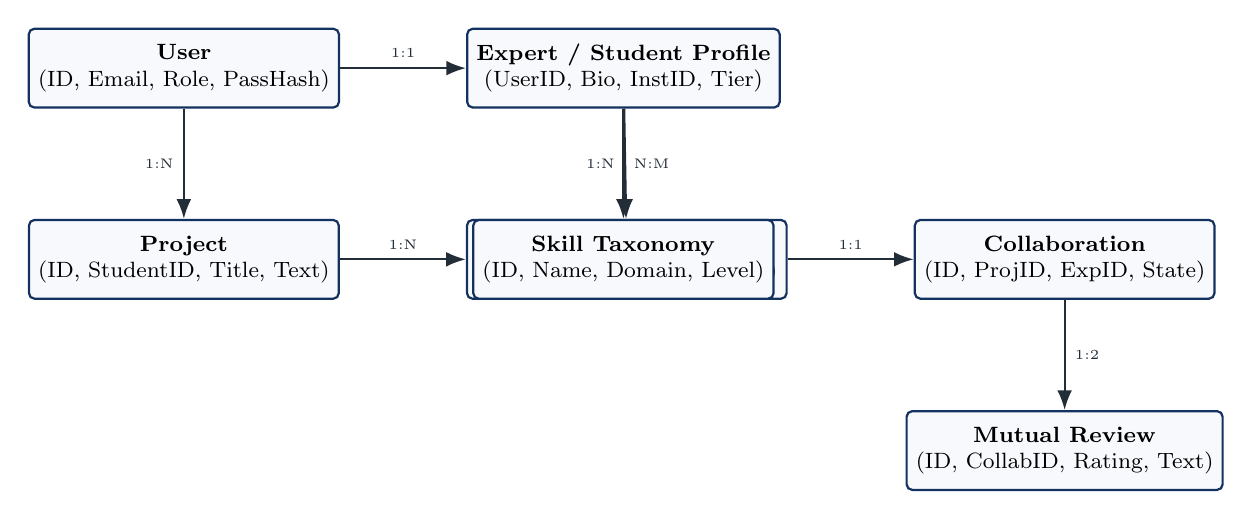
\begin{tikzpicture}[
    entity/.style={rectangle, draw=primary, fill=lightbg, rounded corners=2pt, thick, align=center, font=\footnotesize, minimum height=1.0cm, minimum width=2.4cm},
    rel/.style={-{Latex[length=2.5mm]}, thick, color=darkslate}
]

    \node[entity] (user) {\textbf{User}\\(ID, Email, Role, PassHash)};
    \node[entity, right=1.6cm of user] (profile) {\textbf{Expert / Student Profile}\\(UserID, Bio, InstID, Tier)};
    \node[entity, below=1.4cm of user] (project) {\textbf{Project}\\(ID, StudentID, Title, Text)};
    \node[entity, right=1.6cm of project] (match) {\textbf{Match Score}\\(ProjectID, ExpertID, Score)};
    \node[entity, right=1.6cm of match] (collab) {\textbf{Collaboration}\\(ID, ProjID, ExpID, State)};
    \node[entity, below=1.4cm of profile] (skill) {\textbf{Skill Taxonomy}\\(ID, Name, Domain, Level)};
    \node[entity, below=1.4cm of collab] (review) {\textbf{Mutual Review}\\(ID, CollabID, Rating, Text)};

    \draw[rel] (user) -- node[above,font=\tiny] {1:1} (profile);
    \draw[rel] (user) -- node[left,font=\tiny] {1:N} (project);
    \draw[rel] (project) -- node[above,font=\tiny] {1:N} (match);
    \draw[rel] (profile) -- node[left,font=\tiny] {1:N} (match);
    \draw[rel] (match) -- node[above,font=\tiny] {1:1} (collab);
    \draw[rel] (profile) -- node[right,font=\tiny] {N:M} (skill);
    \draw[rel] (collab) -- node[right,font=\tiny] {1:2} (review);

\end{tikzpicture}%
}
\caption{UniExpert Conceptual Entity-Relationship Diagram}
\label{fig:er_model}
\end{figure}

\subsection{Data Dictionary}
Table~\ref{tab:data_dict} specifies the data dictionary for the core relational tables.

\begin{table}[H]
\centering
\small
\caption{Relational Database Data Dictionary}
\label{tab:data_dict}
\begin{tabularx}{\textwidth}{@{}l l l X@{}}
\toprule
\textbf{Entity / Table} & \textbf{Attribute Name} & \textbf{Data Type} & \textbf{Constraints \& Description} \\
\midrule
\texttt{users} & \texttt{id} & UUID & Primary Key, generated via \texttt{uuid\_generate\_v4()}. \\
& \texttt{email} & VARCHAR(255) & Unique, valid email format, indexed. \\
& \texttt{password\_hash} & VARCHAR(255) & Argon2id hashed password string. \\
& \texttt{role} & ENUM & \texttt{STUDENT}, \texttt{EXPERT}, \texttt{ADMIN}. \\
& \texttt{is\_verified} & BOOLEAN & Default \texttt{FALSE}; set \texttt{TRUE} upon token activation. \\
\addlinespace
\texttt{expert\_profiles} & \texttt{id} & UUID & Primary Key; Foreign Key referencing \texttt{users(id)}. \\
& \texttt{institution} & VARCHAR(255) & Affiliated academic or corporate institution. \\
& \texttt{department} & VARCHAR(255) & Departmental unit or lab name. \\
& \texttt{verification\_tier} & INTEGER & Values $1, 2, 3, 4$ representing badge tier. \\
& \texttt{availability\_status} & ENUM & \texttt{AVAILABLE}, \texttt{LIMITED}, \texttt{BLACKOUT}. \\
& \texttt{max\_active\_load} & INTEGER & Default 3; maximum concurrent collaborations. \\
\addlinespace
\texttt{projects} & \texttt{id} & UUID & Primary Key. \\
& \texttt{student\_id} & UUID & Foreign Key referencing \texttt{users(id)}. \\
& \texttt{title} & VARCHAR(255) & Project working title. \\
& \texttt{raw\_statement} & TEXT & Unstructured proposal text (50--2,000 words). \\
& \texttt{embedding\_id} & VARCHAR(64) & Vector UUID mapped to Qdrant collection point. \\
\addlinespace
\texttt{collaborations} & \texttt{id} & UUID & Primary Key. \\
& \texttt{project\_id} & UUID & Foreign Key referencing \texttt{projects(id)}. \\
& \texttt{expert\_id} & UUID & Foreign Key referencing \texttt{expert\_profiles(id)}. \\
& \texttt{state} & ENUM & \texttt{SUBMITTED}, \texttt{ACCEPTED}, \texttt{ACTIVE}, \texttt{COMPLETED}, etc. \\
& \texttt{created\_at} & TIMESTAMPTZ & Automatically stamped timestamp with timezone. \\
\bottomrule
\end{tabularx}
\end{table}

\clearpage
% ------------------------------------------------------------------------------
% SECTION 7: REQUIREMENTS TRACEABILITY MATRIX
% ------------------------------------------------------------------------------
\section{Requirements Traceability Matrix (RTM)}
\label{sec:traceability}

The Requirements Traceability Matrix (Table~\ref{tab:rtm}) correlates each functional requirement to its design module, test case ID, and verification method. Verification methods are classified per IEEE standard: \textbf{T} (Test), \textbf{D} (Demonstration), \textbf{A} (Analysis), and \textbf{I} (Inspection).

\begin{table}[H]
\centering
\small
\caption{Requirements Traceability Matrix (RTM)}
\label{tab:rtm}
\begin{tabularx}{\textwidth}{@{}l p{4.4cm} l l c@{}}
\toprule
\textbf{Req ID} & \textbf{Requirement Title} & \textbf{Architectural Module} & \textbf{Test Case ID} & \textbf{Method} \\
\midrule
\texttt{FR-AUTH-01} & User Registration \& Verification & Auth Service & \texttt{TC-AUTH-01} & T \\
\texttt{FR-AUTH-02} & Role-Based Access Control (RBAC) & Gateway Service & \texttt{TC-AUTH-02} & T \\
\texttt{FR-PROF-03} & Student Profile Management & Profile Service & \texttt{TC-PROF-01} & D \\
\texttt{FR-PROF-04} & Multi-Tier Credential Verification & Audit Service & \texttt{TC-PROF-02} & I, T \\
\texttt{FR-PROF-05} & Academic Skill Taxonomy & Taxonomy Service & \texttt{TC-TAX-01} & T \\
\texttt{FR-NLP-06}  & Project Statement Ingestion & Project Service & \texttt{TC-PROJ-01} & D \\
\texttt{FR-NLP-07}  & Automated Skill Entity Extraction & AI Inference Engine & \texttt{TC-NLP-01} & A, T \\
\texttt{FR-NLP-08}  & Interactive Requirement Refinement & Web Client UI & \texttt{TC-NLP-02} & D \\
\texttt{FR-REC-09}  & Dense Embedding Generation & AI Inference Engine & \texttt{TC-VEC-01} & T \\
\texttt{FR-REC-10}  & Multi-Criteria Hybrid Scoring & Matchmaking Service & \texttt{TC-REC-01} & A, T \\
\texttt{FR-REC-11}  & Explainable AI Justification & XAI Generator & \texttt{TC-REC-02} & D, T \\
\texttt{FR-REC-12}  & Dynamic Faceted Filtering & Search Service & \texttt{TC-REC-03} & T \\
\texttt{FR-TEAM-13} & Multidisciplinary Decomposition & Team Service & \texttt{TC-TEAM-01} & A, T \\
\texttt{FR-TEAM-14} & Set-Cover Skill Gap Detection & Team Service & \texttt{TC-TEAM-02} & A, T \\
\texttt{FR-TEAM-15} & Side-by-Side Comparison Matrix & Web Client UI & \texttt{TC-TEAM-03} & D \\
\texttt{FR-COL-16}  & Collaboration Lifecycle FSM & Collaboration Service & \texttt{TC-COL-01} & T \\
\texttt{FR-COL-17}  & Anti-Fatigue Quotas \& Blackouts & Governance Service & \texttt{TC-COL-02} & T \\
\texttt{FR-COL-18}  & Secure Workspace \& Messaging & Workspace Service & \texttt{TC-COL-03} & D, T \\
\texttt{FR-GOV-19}  & Structured Peer Review & Reputation Service & \texttt{TC-GOV-01} & D \\
\texttt{FR-GOV-20}  & Admin Verification Dashboard & Admin Service & \texttt{TC-GOV-02} & D, I \\
\bottomrule
\end{tabularx}
\end{table}

\clearpage
% ------------------------------------------------------------------------------
% SECTION 8: VERIFICATION AND VALIDATION PLAN
% ------------------------------------------------------------------------------
\section{Verification and Validation Plan}
\label{sec:vv_plan}

\subsection{Unit and Integration Testing Protocol}
All software components shall be continuously verified within an automated GitHub Actions CI/CD pipeline executing:
\begin{enumerate}[label=\textbf{(\arabic*)},noitemsep]
    \item \textbf{Unit Tests (Pytest):} Minimum 85\% line coverage across backend services, validating mathematical scoring functions, FSM transition integrity, and token parsing.
    \item \textbf{API Integration Tests (HTTPX):} End-to-end testing of REST endpoints ensuring compliance with JSON API schemas and status code contracts.
    \item \textbf{Frontend Component Tests (Jest / React Testing Library):} Verifying accessibility standards and component rendering across edge states.
\end{enumerate}

\subsection{Information Retrieval (IR) Benchmarking Protocol}
The recommendation quality of UniExpert shall be quantitatively validated using a curated benchmark of 50 student research statements with ground-truth expert relevance judgments evaluated by 3 independent academic judges:
\begin{itemize}[noitemsep]
    \item \textbf{Precision at K ($P@K$):} Ratio of relevant experts among the top-$K$ recommendations ($K=3, 5$).
    \item \textbf{Normalized Discounted Cumulative Gain ($NDCG@K$):} Evaluates graded relevance taking position discount into account.
    \item \textbf{Comparative Baselines:} Performance of the Hybrid Engine (Eq.~\ref{eq:srs_hybrid}) shall be compared directly against BM25 lexical keyword matching and isolated dense vector retrieval.
\end{itemize}

\subsection{User Acceptance Testing (UAT)}
A formal UAT phase will be conducted in December 2026 involving a cohort of 20 university students and 8 faculty advisors. Test scenarios will cover: (1) project submission; (2) reviewing recommendations; (3) sending collaboration proposals; and (4) evaluating workspace utility. Success is defined as achieving a task completion rate $\ge 90\%$ and an average SUS score $\ge 80$.

\vspace{0.8cm}
% ------------------------------------------------------------------------------
% SECTION 9: COMMITTEE SIGN-OFF & APPROVAL
% ------------------------------------------------------------------------------
\section{Committee Review and Sign-Off}

By signing below, the supervisor and capstone examination committee confirm that this Software Requirements Specification (SRS) establishes the approved functional, architectural, and evaluation scope for the \textbf{UniExpert} Capstone Project for the Fall 2026 academic semester.

\vspace{1.0cm}
\noindent
\begin{minipage}[t]{0.48\textwidth}
    \rule{2.8in}{0.6pt}\\[0.2cm]
    \textbf{Mr. Md. Shohel Arman}\\
    Assistant Professor\\
    Department of Software Engineering\\
    Faculty of Science \& Information Technology\\
    \textit{Date:} \rule{1.5in}{0.4pt}
\end{minipage}
\hfill
\begin{minipage}[t]{0.48\textwidth}
    \rule{2.8in}{0.6pt}\\[0.2cm]
    \textbf{Head of Department / Committee Chair}\\
    Department of Software Engineering\\
    Faculty of Science \& Information Technology\\
    \textit{Date:} \rule{1.5in}{0.4pt}
\end{minipage}

\end{document}
